\chapter{Introduzione}\label{cap:introduzione}

\section{Contesto}\label{sez:contesto}

In seguito alla crescita esponenziale del web in questo secolo e con l'abituarsi di tutti coloro che ne usufruiscono ad un livello grafico sempre migliore e ad una esperienza mano a mano pi\`u interattiva e studiata per l'utente medio, le tecnologie utilizzate per costruire i siti web si sono adattate per permettere uno sviluppo sempre pi\`u rapido di codice pi\`u facilmente testabile e mantenibile.

Di conseguenza nel frontend si sono susseguiti una serie di framework e di strumenti in modo molto rapido, a partire da JQuery\cite{jquery} nel 2006, che per primo si \`e occupato di risolvere il problema della compatibilit\`a del codice scritto con i diversi browsers, permettendo ai developers di scrivere una volta, e poter eseguire su tutti i pi\`u diffusi.

Nel 2010 \`e stato creato AngularJS, il primo framework per applicazioni che seguono il pattern architetturale Model-View-Controller(MVC) ad offrire in un unico pacchetto un insieme di features che hanno facilitato molto la vita agli sviluppatori, come il two-way data binding, la dependency injection, il routing integrato, ed altri strumenti utili per rendere pi\`u standard lo sviluppo nel frontend~\cite{Hoff}.
AngularJS pur essendo stato largamente utilizzato, \`e stato cambiato radicalmente nel 2013 e rinominato in Angular2 (e nelle versioni pi\`u recenti semplicemente Angular) senza mantenere retrocompatibilit\`a e senza offrire un modo preciso per migrare alla nuova versione ai precedenti utilizzatori di AngularJS.
Anche per questo motivo, React, un altro framework pi\`u leggero e modulare mantenuto da Facebook e la cui prima versione risale al 2013, ha poco a poco preso il posto di Angular come framework pi\`u utilizzato dai developers nel frontend, visibile anche nell'ultimo questionario condotto dal sito StackOverflow nel quale \`e stato chiesto quali tecnologie vengano utilizzate a circa 90000 sviluppatori in tutto il mondo\cite{stackOverflow2019}.
Infine Vue, lanciato nel 2014, \`e il terzo dei principali framework moderni per la creazione di interfacce utente ed \`e stato fortemente adottato, proponendo una versione intermedia tra il pi\`u opinionato Angular e il pi\`u flessibile React\cite{vueJs}.

Oltre ad almeno uno dei framework citati, ciascuno con la propria semantica, organizzazione logica delle cartelle e spesso una CLI dedicata, un frontend developer odierno dovrebbe conoscere bene HTML, CSS e chiaramente Javascript, jQuery per retrocompatibilit\`a ed almeno Bootstrap per creare componenti standard pi\`u in fretta.

In particolare se si utilizza Angular, come anche se si vuole scrivere codice pi\`u facilmente mantenibile e type-safe, il developer dovr\`a conoscere anche TypeScript.
TypeScript \`e un linguaggio di programmazione che estende la sintassi di Javascript, rendendolo tipizzato(e non interpretato), e viene quindi compilato e trasformato in codice equivalente nel linguaggio javascript, per poter essere utilizzato dal browser.
Questo processo di compilazione e traduzione da un linguaggio verso l'altro, prende il nome di transpilazione.

\section{Problema}\label{sez:problema}
I continui aggiornamenti nei molti framework utilizzati e la diversit\`a degli strumenti tra loro, che spesso realizzano in modo diverso la stessa cosa, rendono sempre pi\`u difficile per un junior developer iniziare a sviluppare, vista l'ampia curva di apprendimento e quindi il tempo e lo studio necessario, per poter essere pronto a lavorare come professionista.

Spesso i web developer infatti finiscono per scegliere se diventare uno sviluppatore frontend e concentrarsi su quello stack di tecnologie da conoscere ed approfondire, o se diventare un developer backend, dato che rimanere al passo anche solo uno di questi due campi richiede tempo, oltre all'impegno.

\`E quindi chiaro che da parte di tutti i web developer e specialmente per una figura esperta e mista identificata con il titolo "Full-Stack Developer", ci sia una continua ricerca del modo per rendere le proprie competenze quanto pi\`u trasversali possibile, anche in termini di tecnologie utilizzate.

\pagebreak

\section{Linguaggi General-Purpose}\label{sez:linguaggiGeneralPurpose}
Microsoft, nel backend e in ambito applicativo, ha reso nel tempo il framework .NET Standard e le sue implementazioni(la piattaforma .NET Core, il .NET Framework e Mono) utilizzabili nei vari linguaggi sviluppati da Microsoft ovvero C\#, F\# e VB.
La figura \ref{fig:DotNetImplementations} di seguito riassume le implementazioni del .NET Standard e le varie tipologie di applicazioni che si possono sviluppare con ciascuna.

\begin{figure}[H]
	\centerline{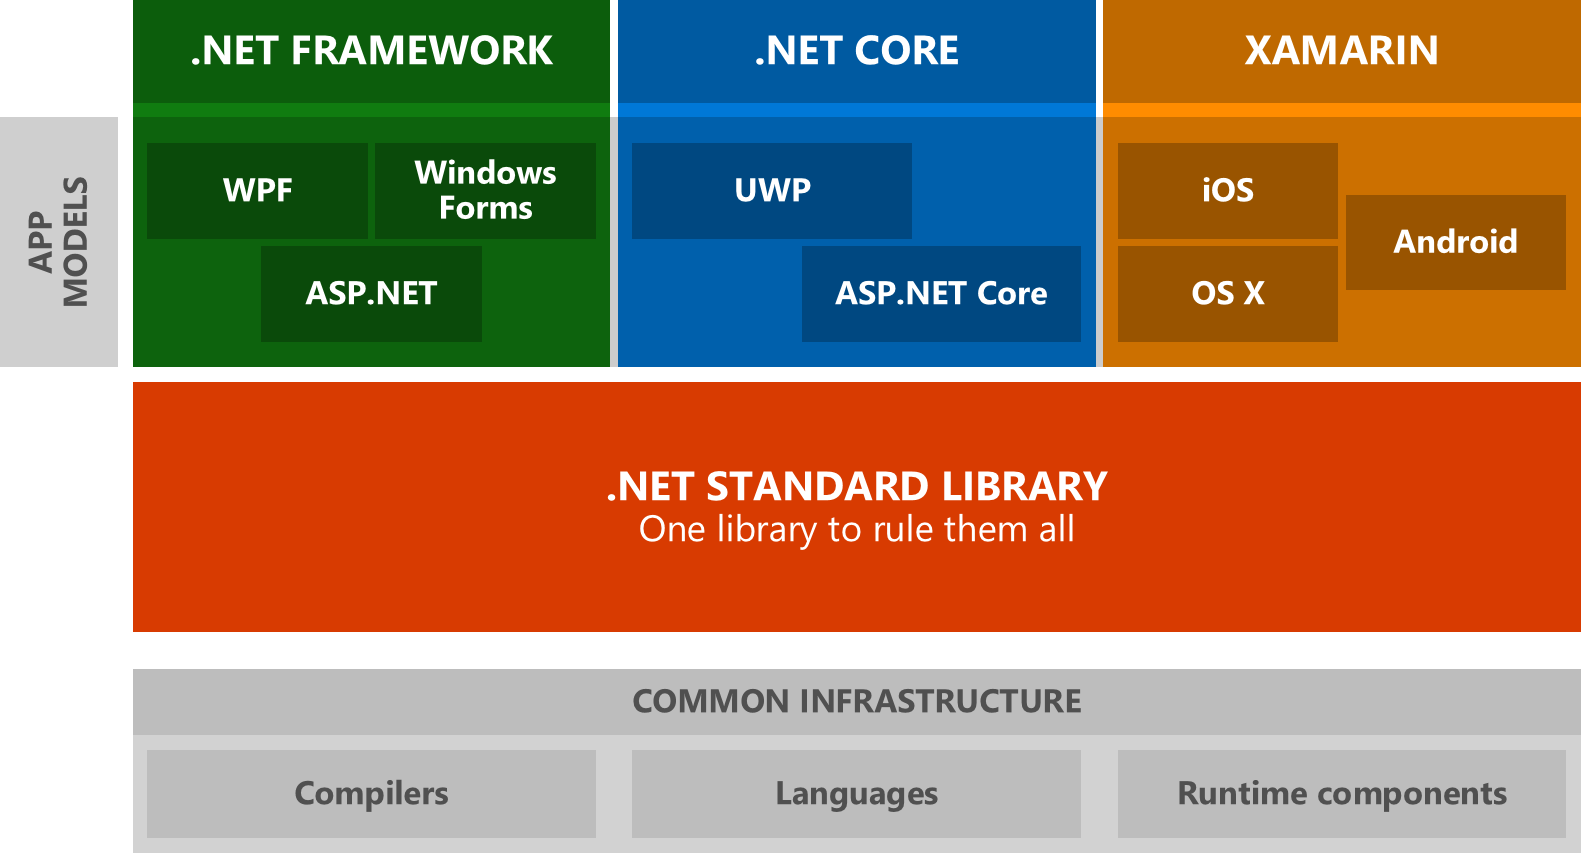
\includegraphics[scale=0.2]{figure/DotNetImplementations}}
	\caption{Implementazioni del .NET Standard}
	\label{fig:DotNetImplementations}
\end{figure}

Se si decide di sviluppare codice per un'applicazione web che gestisca eventi del Browser con prestazioni native(click, drag, hover,...) e non si vuole costringere gli utenti che la dovranno utilizzare a scaricare dei plugin, si \`e costretti a scriverla utilizzando Javascript(JS).
Eventualmente sfruttando anche un framework basato su JS se si vuole essere pi\`u veloci nello sviluppo e scrivere codice mantenibile, esigenze fondamentali a livello enterprise.

\begin{figure}[H]
\centerline{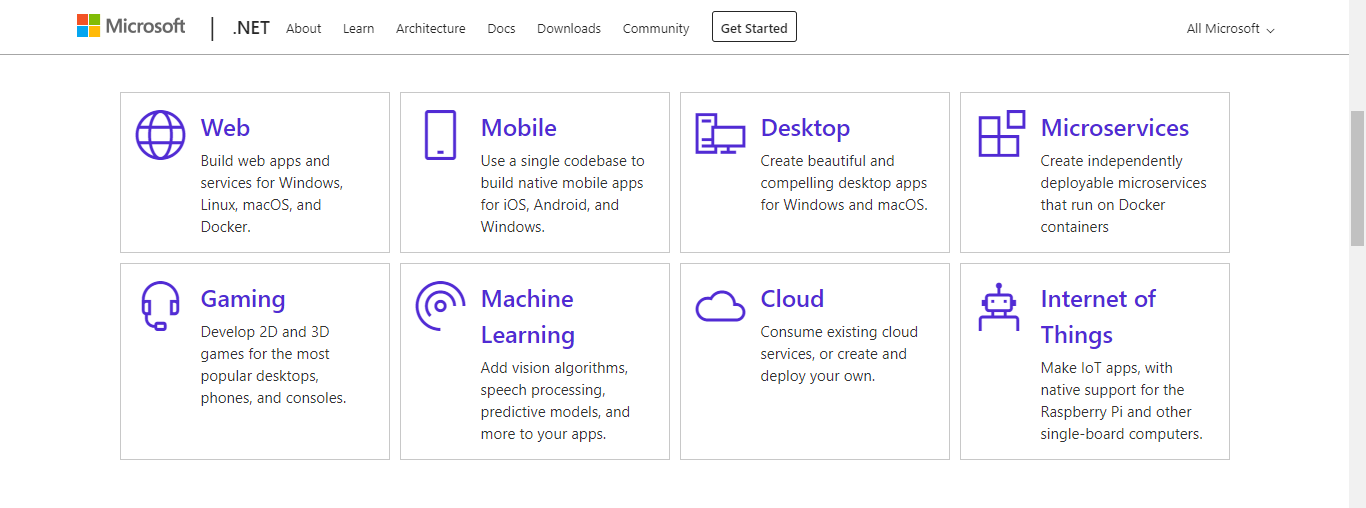
\includegraphics[scale=0.35]{figure/DotNetFrameworkCapabilities}}
\caption{Possibilit\`a di .NET}
\label{fig:DotNetCapabilities}
\end{figure}

Gi\`a con il rilascio di Razor\cite{razor} nel 2011, Microsoft ha permesso la generazione di codice HTML e CSS in modo dinamico utilizzando C\#, ma questa tecnologia \`e stata creata e pensata per il server-side rendering ed \`e quindi utilizzabile solo quando si scrive codice che sar\`a eseguito da un server, non da un browser.
Ci\`o implica che la cattura di un evento client side come il click di un utente su un bottone, senza dover eseguire una chiamata al server sul quale viene eseguito l'hosting dell'applicazione e l'attesa della relativa una risposta, non risulti possibile senza l'utilizzo di JS.

\section{Blazor}
Ecco cosa \`e quindi Blazor: la versione pi\`u avanzata di Razor(Browser+Razor\cite{blazorWikiGitHub}), o meglio un Framework per la creazione di User Interfaces(UI) di Single Page Application(SPA) che permette ai developer di gestire anche gli eventi client-side, sviluppando in C\# o nel linguaggio scelto tra quelli supportati.
Per SPA si intende un applicazione web che interagisce con l'utente riscrivendo dinamicamente la pagina nel quale l'utente si trova a seconda delle sue azioni, piuttosto che ricaricare nuove pagine di volta in volta richiedendole al server ad ogni click\cite{SPA}.
Questo framework permette allo sviluppatore di scrivere codice come se il linguaggio scelto(non JS) fosse effettivamente ci\`o che viene eseguito dal client, mentre in realt\`a ci\`o che viene eseguito dal browser dell'utente cambia a seconda del modello scelto, come poi vedremo pi\`u nel dettaglio.

Blazor utilizza per i vari modelli, delle tecnologie diverse che rispettano lo standard del web, in quanto non sfrutta componenti che ogni utente deve appositamente scaricare per poter utilizzare l'applicazione, e non dipende da un browser specifico.

Lo scopo di questa tesi \`e quindi di provare a spiegare che cosa sia Blazor, come e perch\`e funzioni diversamente nei suoi vari modelli, spiegare come mai non esiste un unico modello mettendo a confronto quelli disponibili e provando a trovare il migliore, se ne esiste uno.